\section{Appendix A: Figures}

\begin{figure}[H]
\begin{center}
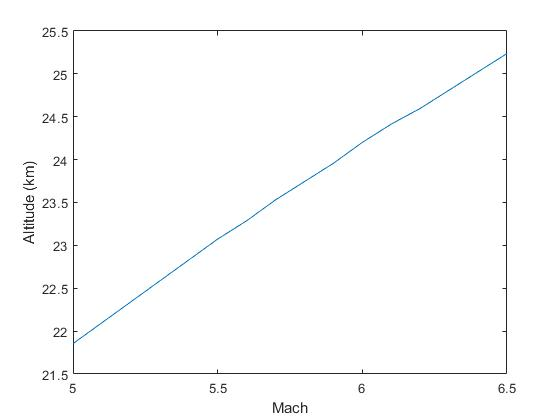
\includegraphics[width=0.6\textwidth]{altVMach}
\caption{Altitude v. Mach}
\label{fig:altVMach}
\end{center}
\end{figure}

\begin{figure}[H]
\begin{center}
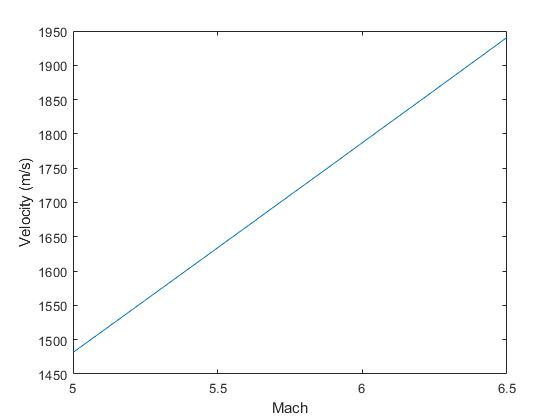
\includegraphics[width=0.6\textwidth]{velVMach}
\caption{Velocity v. Mach}
\label{fig:velVMach}
\end{center}
\end{figure}

\begin{figure}[H]
\begin{center}
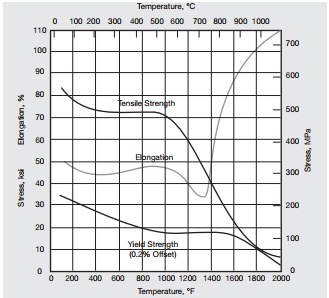
\includegraphics[width=0.6\textwidth]{incoloyPlot}
\caption{Temperature Range Across Combustor Structure \cite{inco}}
\label{fig:incoloyPlot}
\end{center}
\end{figure}

\begin{figure}[H]
\begin{center}
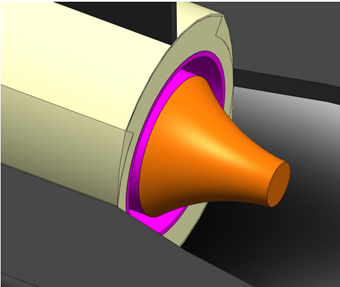
\includegraphics[width=0.5\textwidth]{nozzleIsoView}
\caption{Final Nozzle Design}
\label{fig:nozzleIsoView}
\end{center}
\end{figure}

\begin{figure}[H]
\begin{center}
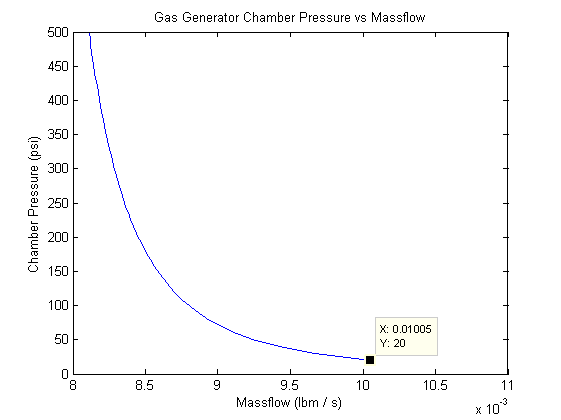
\includegraphics[width=0.6\textwidth]{turboPressureVMdot}
\caption{Turbopump Pressure v. Mass Flow Rate}
\label{fig:turboPressureVMdot}
\end{center}
\end{figure}


\begin{figure}[H]
\begin{center}
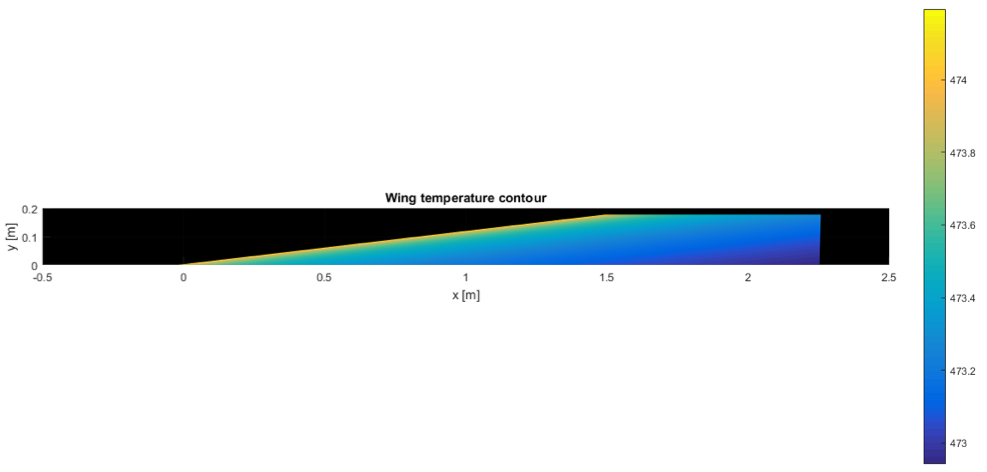
\includegraphics[width=\textwidth]{wingTemps}
\caption{Wing Surface Temperature Plot}
\label{fig:wingTemps}
\end{center}
\end{figure}


\newpage
\section{Appendix B: Equations}

\begin{equation}
\begin{split}
Re_x=\frac{\rho u x}{\mu}	\\
\text{If } Re_x<500,000, \text{ Laminar boundary layer} \\
\text{If }   Re_x>500,000, \text{ Turbulent boundary layer}
\end{split}
\label{eqn:reynolds}
\end{equation}


\begin{equation}
Pr=\frac{\mu Cp}{K}
\label{eqn:prandtl}
\end{equation}

\begin{equation}
Nu_x=\frac{h_g x}{K}
\label{eqn:nusselt}
\end{equation}

\newpage
\section{Appendix C: Air Properties}
\begin{figure}[H]
\begin{center}
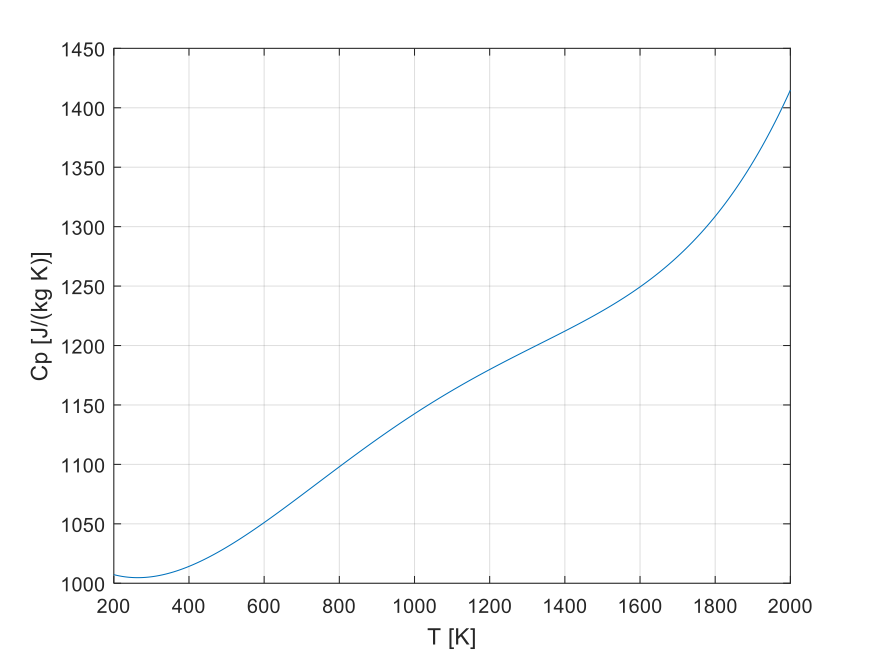
\includegraphics[width=0.7\textwidth]{airCpvT}
\caption{Specific Heat v. Temperature for Air}
\label{fig:airCpvT}
\end{center}
\end{figure}


\begin{figure}[H]
\begin{center}
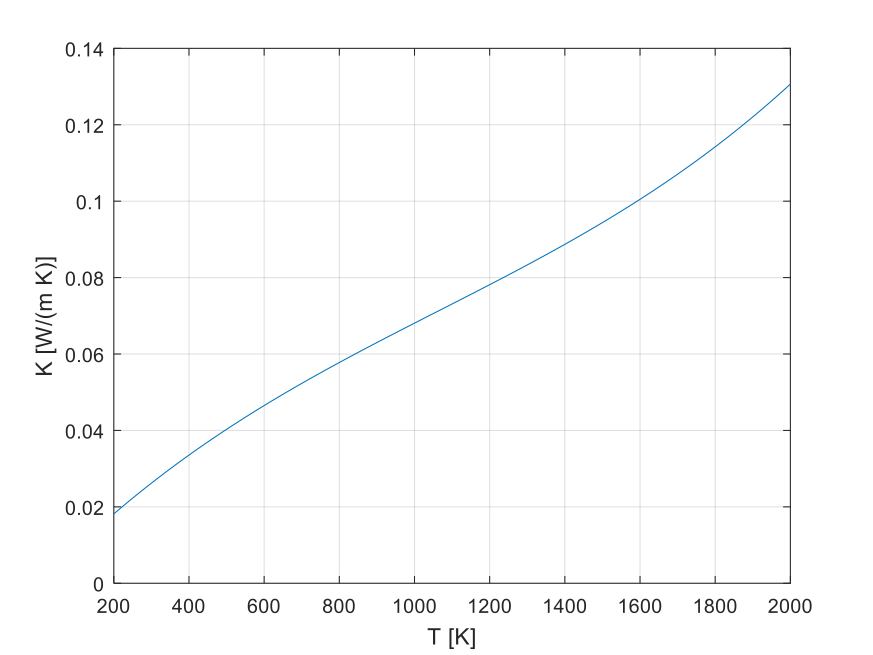
\includegraphics[width=0.7\textwidth]{airKvT}
\caption{Conduction Heat Transfer Coefficient v. Temperature for Air}
\label{fig:airKvT}
\end{center}
\end{figure}

\begin{figure}[H]
\begin{center}
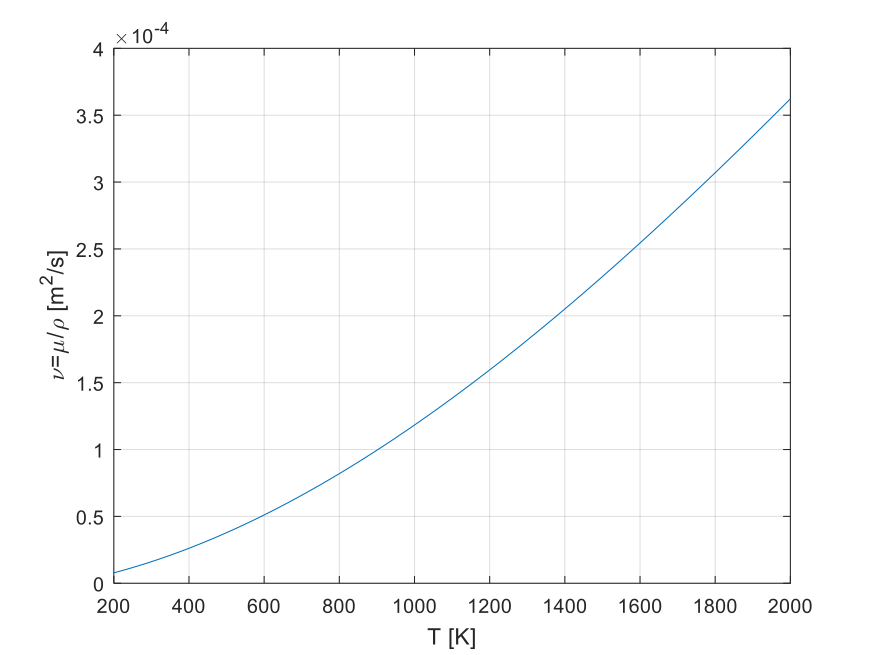
\includegraphics[width=0.7\textwidth]{airNuvT}
\caption{Kinematic Viscosity v. Temperature for Air}
\label{fig:airNuvT}
\end{center}
\end{figure}

\newpage
\section{Appendix D: Chapman-Jouguet Detonation Model}
\textit{This page intentionally left blank}

\newpage
\section{Appendix E: Alternative RDE Analysis Model}
\textit{This page intentionally left blank}

